%!TEX root = ../thesis.tex
% \title{Kinectograph: Body-Tracking Camera Control for Self-Directed Demonstration Videos}
\chapter{Kinectograph: Body-Tracking Camera Control}
\label{chapter_kinectograph}

A large community of users creates and shares how-to videos online. Many of these videos show demonstrations of physical tasks, such as fixing a machine or demonstrating dance steps. It is often difficult for the authors of these videos to control camera focus, view, and position while performing their tasks.

To help instructors produce videos, in this chapter, we introduce Kinectograph\footnote{This work was published at CHI 2013~\cite{Cheng:2013:BCC:2468356.2468568}.}, a recording device that automatically pans and tilts to follow specific body parts, e.g., hands, of a user in a video with lightweight control. It utilizes a Kinect depth sensor to track skeletal data and adjusts the camera angle via a 2D pan-tilt gimbal mount. Users configure Kinectograph through a tablet application with real-time video preview. We conducted a preliminary evaluations to test the usability of Kinectograph's control interface. All of the participants successfully created instructional videos without assistance. The initial findings suggested that Kinectograph enables instructors to focus on performing their demonstrations, while giving them sufficient camera control at recording time.

%!TEX root = ../thesis.tex
\section{Introduction}

Popular online video-sharing websites such as YouTube have enabled the growth of a large community of users who share their knowledge and expertise in video tutorials. How-To videos demonstrate specific skills and procedures for tasks as varied as cooking, building a treehouse, or fixing a machine \cite{Torrey:2007he}.
These online tutorials help learners observe the manipulations and then put them into practice \cite{Torrey:2009fc}. However, in recording these videos, instructors often find it challenging to control the camera during demonstration.
%
Working with a cameraman who controls the device and viewpoints ensures that the video captures the movements that the audience would want to see, but it requires having a second person to direct the recording and work closely together with instructors. Many amateur users who mostly work alone, therefore, choose to self-record with one or more cameras. Camcorders can be set on a tripod to capture a static viewpoint, but it is hard to make sure whether users' actions are properly in frame at recording time. An alternative is to wear a head mounted camera to record what the instructors see. This may record unwanted and distractive head movements, making it difficult for the audience to watch. Additional camera views of the overall workspace might be needed to assist learners with understanding the context of demonstrated actions \cite{Fussell:2003te}.

\begin{figure}[t]
\centering
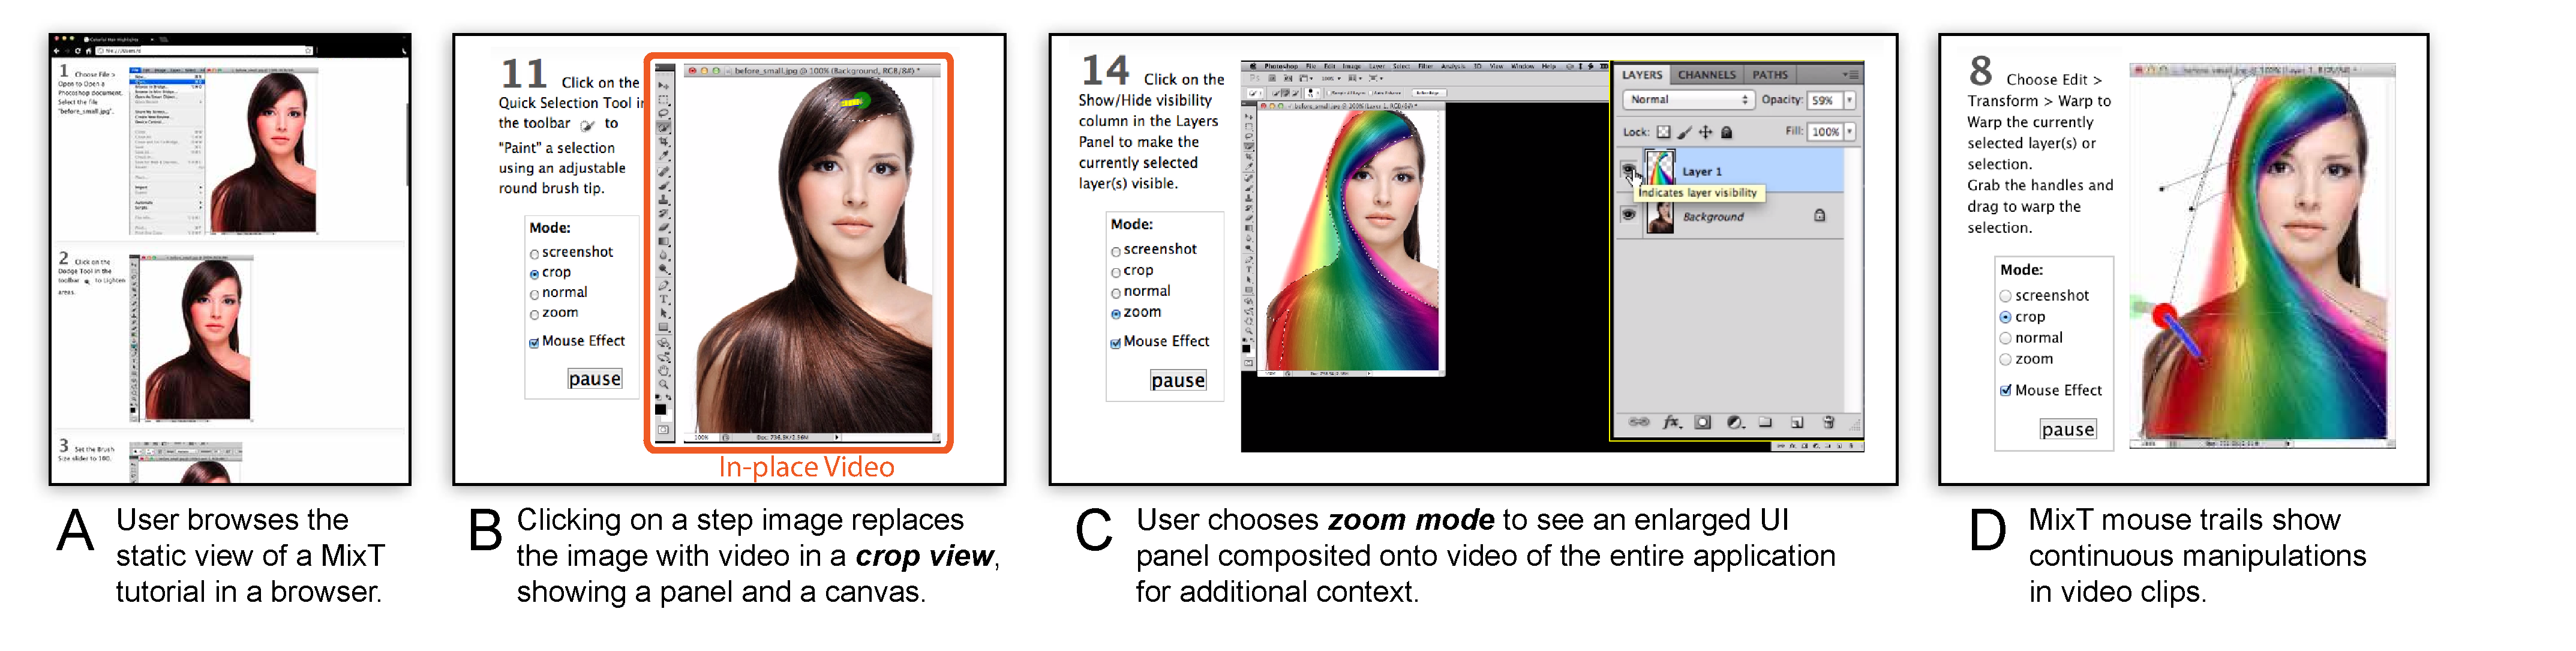
\includegraphics[width=0.8\columnwidth]{\kinectograph/fig/teaser.pdf}
\caption{Kinectograph includes a Kinect camera to track user movement and a motorized dock to pan and tilt the camera so that the user (or their hand) remains centered in the recorded video. Here the device follows the user\'s hand while he is illustrating.}
\label{fig:figure1}
\end{figure}

Seeing these filming challenges, we would like to enable users to gain the flexibility of real-time camera control without requiring a dedicated camera-person. Our goal is to design a device that can automatically track and orient to film the tutorial instructors while providing lightweight manual controls. Existing video conferencing cameras and surveillance tools offer human tracking to provide full or partial automatic viewpoint control. Polycom\footnote{http://www.polycom.com/} designs video conferencing cameras that feature face recognition and voice detection to enable a group of users to talk in an office room setting. This approach assumes people's faces should be in the frame, which may not be true for instructional videos that focus on actions rather than ``talking heads.''
%
Automatic motion tracking is possible to always keep the user in view using visible markers \cite{Ranjan:2010} or wearable sensors such as infrared emitters by Swivl\footnote{http://www.swivl.com/}. However, instructors are unlikely to take such approaches to put on visible markers when demonstrating.
%
Researchers have been developing techniques to track specific targets using computer vision, including hands \cite{Ranjan:2008}, user movements \cite{Wilson:2012fb}, fast-moving objects (e.g., a Ping-Pong ball) \cite{Okumura:2011tr}, or regions in pre-defined spaces \cite{Ranjan:2007}. These usually require an expert defining heuristics of space regions or movement classifications ahead of time for the tracking program. On the contrary, we aim at proposing a new approach that does not have these issues, gives users flexibility in a home environment, and provides interactive control over the behavior of the camera tracking.
%
% TeleAdvisor assists a helper to remotely observe a physical task in real-time and provide instructions~\cite{Gurevich:2012ko}. However, the system is limited by the static camera view without automatic tracking.
%

\clearpage
We propose Kinectograph, a new device that enables semi-automatic camera control for users to self-direct camera orientation for demonstration tasks (Figure~\ref{fig:figure1}). Kinectograph serves as both the camera and the cameraman. It provides a motorized dock for a Kinect\footnote{http://www.xbox.com/en-US/kinect} sensor and a tablet-based user interface (separate from the camera) to switch between tracking regions at runtime based on their needs when demonstrating. Using skeleton tracking to follow the user’s movement, Kinectograph automatically pans and tilts the camera in real time. Users can define zoom regions that follow his actions to provide closeup views. Using a Kinect sensor, our system works in a common indoor setting and does not require the user to wear sensors or configure the environments. Kinectograph makes a novel contribution over the prior art in its mixed-initiative approach that offers various levels of automation and control to users at record time.

In the following section (Section \ref{kinectograph_authoring}), we describe the user experience of recording with Kinectograph. We also describe design and implementation decisions (Section \ref{kinectograph_tracking}). Finally, in Section \ref{kinectograph_study}, we review findings from a preliminary evaluation with 7 participants to study Kinectograph's usability of self-recording tutorials. All of the participants successfully created a demonstration video using our system without assistance and found it easy to interact with.

%\bjoern{I cut this out because you are missing the reference.}\new{In [insert citation here], they similarly use motors and a camera to automatically track and zooming in on users, but they do so in a conference setting. One of their system objectives is to unobtrusively track; however, our system focuses on providing enabling user's control in these tracking and zooming decisions for their DIY tutorials. In addition they only use facial and audio tracking and do not leverage the power of the kinect to do skeletal tracking.}

% Abhishek Ranjan, Jeremy Birnholtz, Rorik Henrikson, Ravin Balakrishnan, Dana Lee. (2010). Automatic camera control using unobtrusive vision and audio tracking. Proceedings of GI 2010 – the Graphics Interface Conference. p. 47-54.
%\pc{Where is the reference to the papers Bjoern sent? auto-tracking camera}


%!TEX root = ../thesis.tex
\section{Authoring}
% \section{Recording with Kinectograph}
%\bjoern{moved to intro}Kinectograph serves as both the camera and the cameraman. It provides a motorized dock for a Kinect sensor and a tablet-based user interface (separate from the camera) to control the camera orientation (Figure 1). By using the Kinect to track the user’s movement, Kinectograph automatically pans and tilts the camera in real time. The portable size of Kinectograph makes it easy to be placed on a tabletop surface or a TV stand to capture the room where the user will perform.

\begin{figure}[t]
\centering
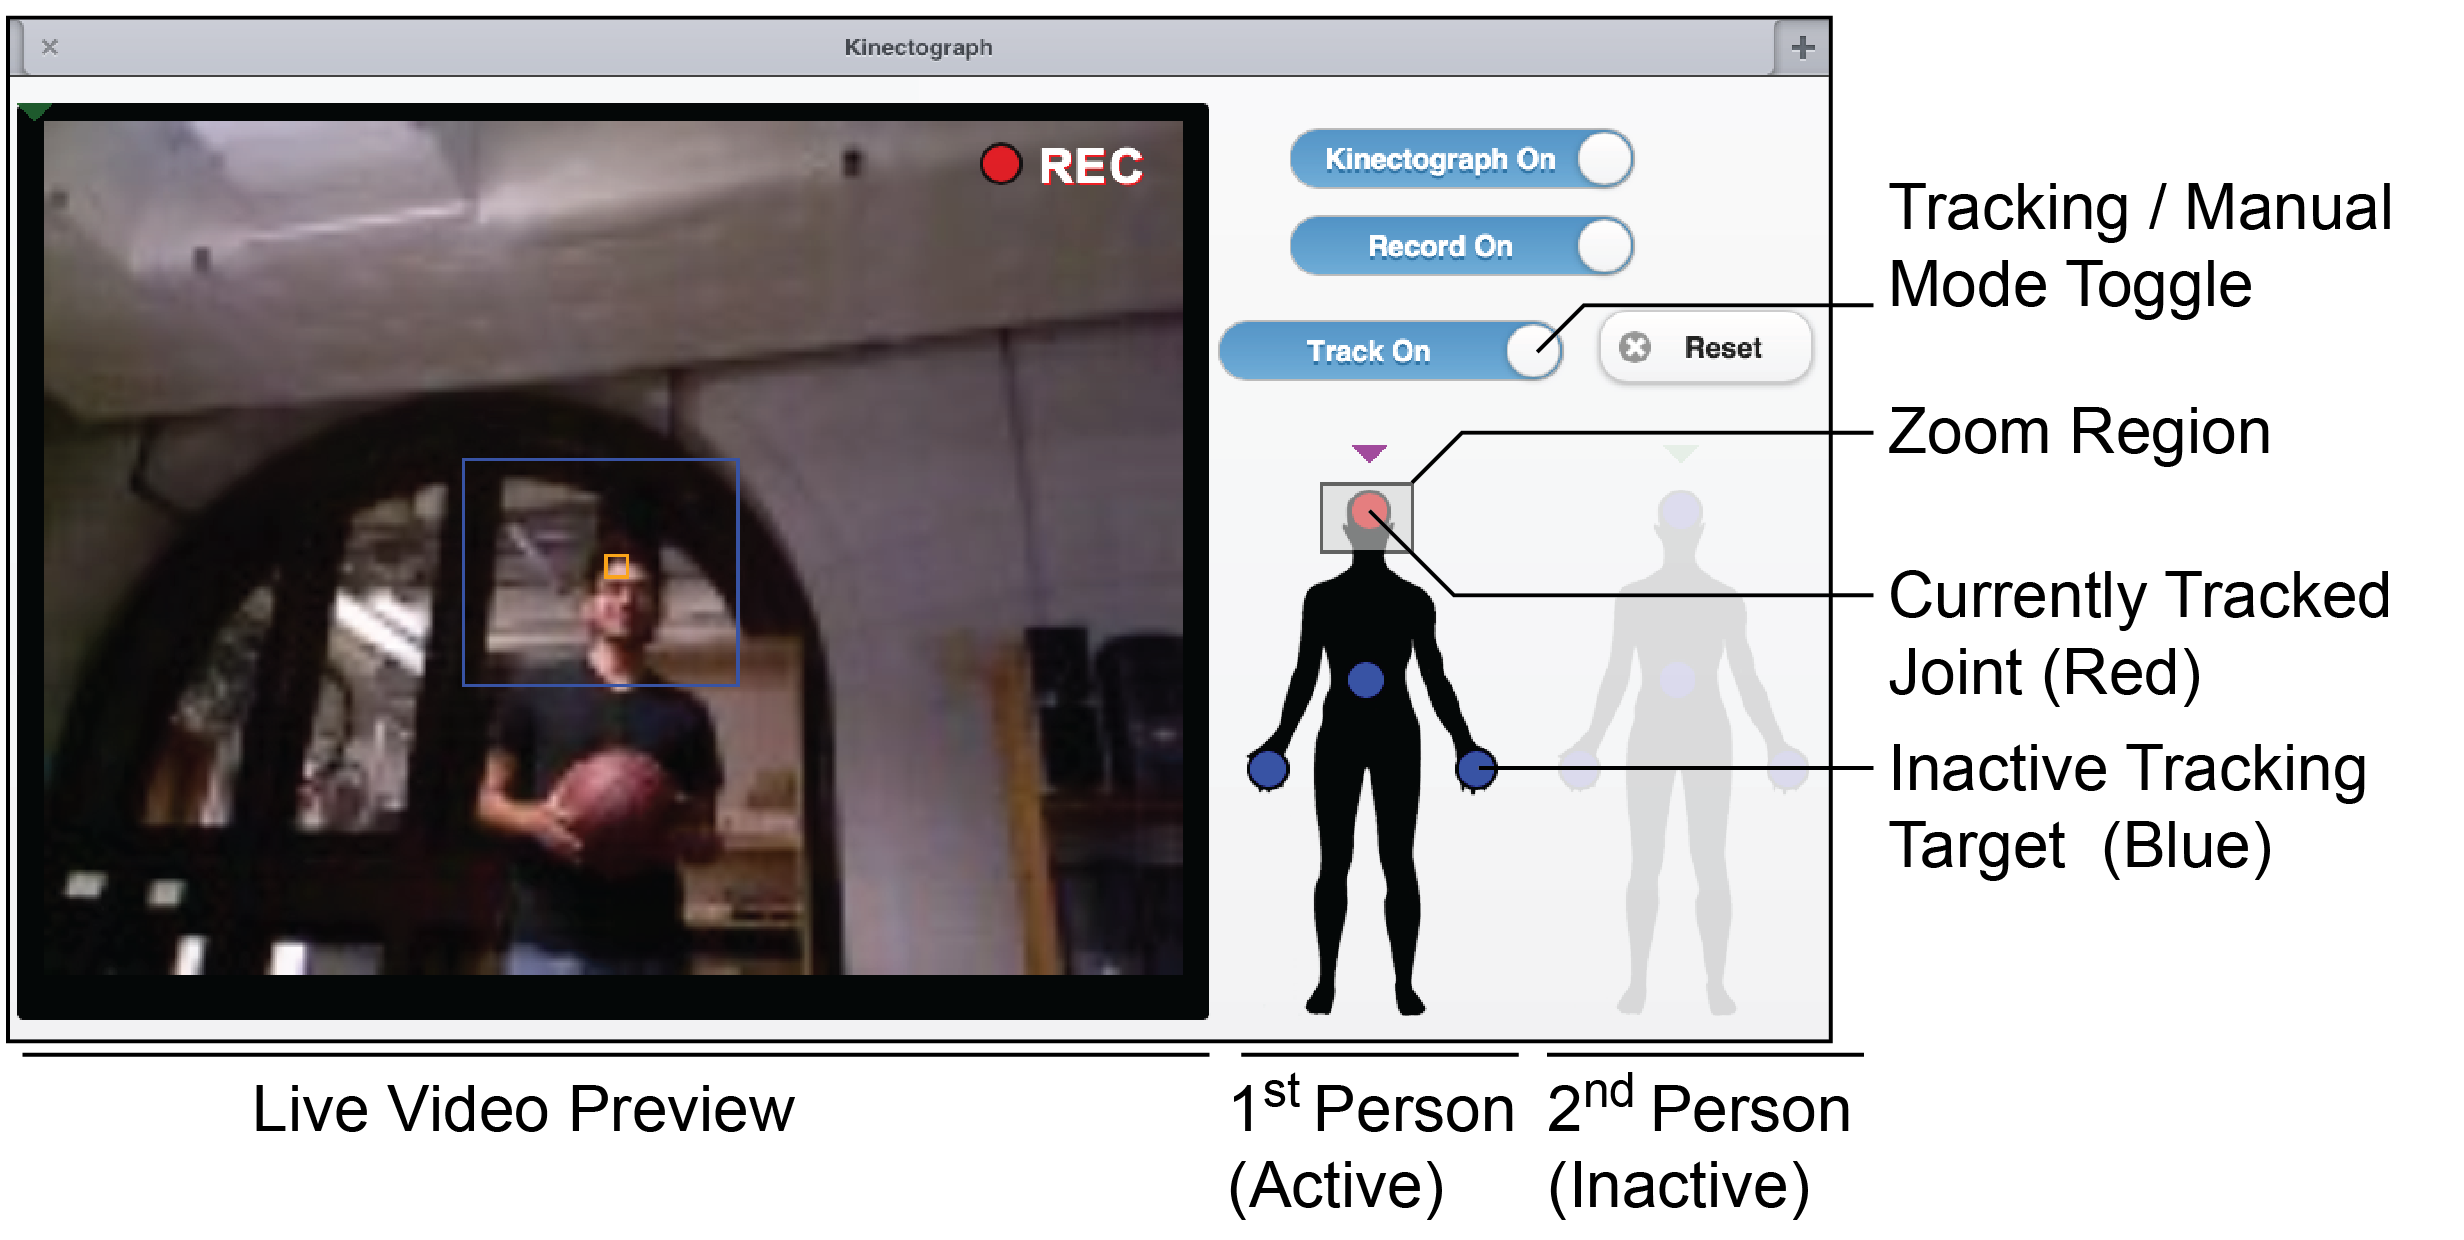
\includegraphics[width=1.0\columnwidth]{\kinectograph/fig/newui}
\caption{Kinectograph UI on a tablet device}
\label{fig:figure4}
\end{figure}

Users connect the Kinectograph device to a personal computer and start its server software, then open the Kinectograph mobile control UI (Figure \ref{fig:figure4}) on a phone or tablet that they can carry with them during their demonstration.
% \bh{You had an architecture figure at some point. Where did it go?}
%
In order to allow How-To tutorial makers as much control over the filming of their tutorial with as little effort as possible, Kinectograph offers the following features on its mobile control UI:

\subsection{Real-time Video View}
In a self video recording, it is convenient for the user to be able to view the current state of their video to make filming decisions. Thus, Kinectograph's UI displays a real-time video feed (currently limited to a low fps) from the Kinect camera.

\subsection{Manual Control}
Users can manually control the camera angle by swiping on the preview image to pan and tilt the camera. For example, during a cooking demonstration, users may wish to pan to a shot of the oven to their left or the sink to their right, or tilt down when they open the oven.
% We share this interaction technique with robotic telepresence systems (e.g. Revolve Robotics' Kubi \footnote{http://www.revolverobotics.com/}). %\bh {does zoom work in manual mode? I don't know how.}

\subsection{Automated Tracking Control}
Demonstrations may require users to move around, such as in furniture assembling or personal training videos. Kinectograph's automated tracking control enables users to focus on their demonstration. Thus, users can switch to automatic camera mode to have Kinectograph track them. Kinectograph can follow one or two actors. Users select which body parts should remain in the frame by tapping on targets of an iconic body outline in the UI - e.g., the head (as in video conferencing systems) or the hands (which may be more important for demonstrations). To keep the entire upper body in view, users can select multiple joints simultaneously. Each selected joint can be deselected by toggling the target button on the iconic body outline.

Early testing showed that because the video feed to the tablet has some latency and a lower framerate, selecting joints on the video feed itself can be difficult if those joints are moving. We therefore chose to display a static, iconic body outline.
%display an iconic body outline next to the video feed on the UI to give users a static target for activating and deactivating joint tracking.

%An indicator marker is overlaid on the realtime view to show where where the camera will center (e.g., if multiple joints are tracked, the center of those joints will be displayed). \bjoern{don't need this i think}

\subsection{Zoom Control}
Close-ups of important steps are a common editing technique in demonstration videos. To capture close-ups, users can define a zoom region related to their body by dragging a rectangular area across the iconic body outline - e.g., they can draw a region that captures their hands to focus on their hand motions. Because the camera used has a fixed focal length, our current prototype uses digital zoom (Figure~\ref{fig:ZoomView}). By default any joints in the zoomed region are automatically added to the track list.

\subsection{Reset}
Finally, the UI provides a button to dismiss any joints selected for automated tracking or for zooming.

\begin{figure}[t]
\centering
\includegraphics[width=1\columnwidth]{\kinectograph/fig/ZoomView}
\caption{Kinectograph tracks and provides a digital zoom view (right) captured from the Kinect camera view (left) in real-time based on user specified area.}
\label{fig:ZoomView}
\end{figure}

\begin{figure}[t]
\centering
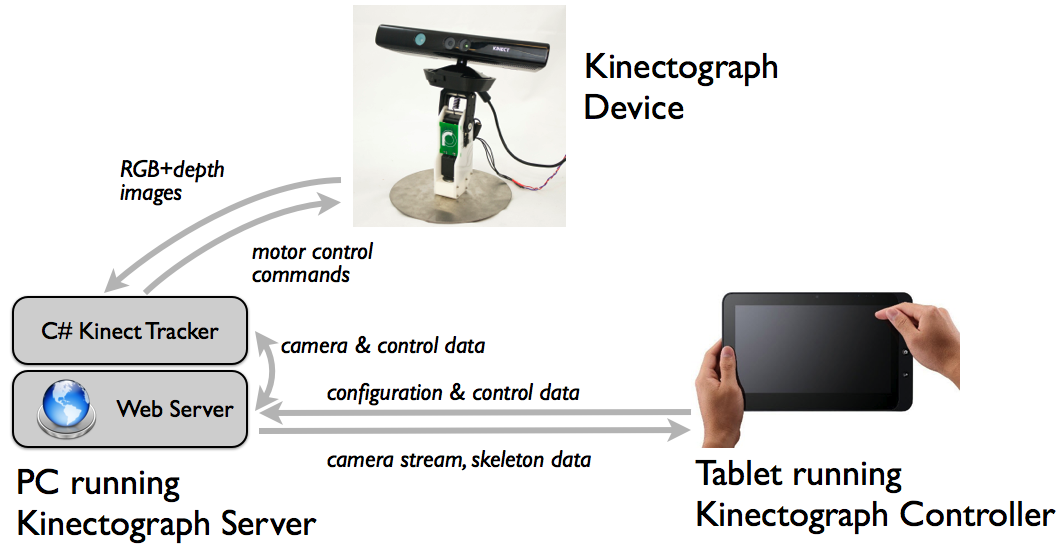
\includegraphics[width=1.0\columnwidth]{\kinectograph/fig/arch.png}
\caption{Kinectograph Architecture}
\label{fig:architecture}
\end{figure}


%!TEX root = ../thesis.tex
\section{Computer-Generated Visualization}

\subsection{Augmented Workflow}
For presenters to narrate ``live'' over a video recording, we propose augmenting a typical workflow from capturing a screencast video; to rehearsing it and adjusting timings; and finally to live presentation of the demo video (Figure~\ref{fig:demowiz_workflow}).

DemoWiz first captures a screencast video and input events during a software demonstration from a user-defined rectangular region. Once the recording is done, DemoWiz analyzes the low-level event stream and transforms it into higher-level events such as mouse clicks, double-clicks, and drags. DemoWiz then allows presenters to edit the timing and notes while practicing their presentations with the presenter view equipped with an adjustable event timeline (Figure~\ref{fig:demowiz_teaser}A). Finally, presenters can give a live presentation using the same UI (i.e., presenter view) and show the audience view without visualization to the viewers.

\begin{figure*}[t]
  \centering
  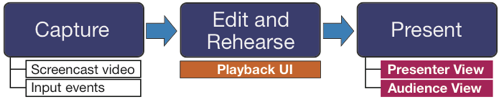
\includegraphics[width=0.7\textwidth]{\demowiz/fig/demowiz_workflow}
  \caption{DemoWiz workflow: Presenters captures a software demonstration, edit the video recording while rehearsing with our playback UI, and present the edited video to the audience using a presenter view.}
  \label{fig:demowiz_workflow}
\end{figure*}

% ---------------------------------------------------------------

\subsection{Visualizations}
To enable presenters to focus on their narration and the original video contents, DemoWiz augments the screencast recording by automatically overlaying simple glyphs.

\subsubsection{Input Event Glyphs}
DemoWiz overlays visual annotations of events on the screencast recording in a graphical way where the events happen.For example, in Figure~\ref{fig:demowiz_teaser}, the presenter clicks and drags the map view to the right. DemoWiz uses the following simple,distinctive glyphs to differentiate event types as Figure~\ref{fig:demowiz_glyphs} shows:

\begin{itemize}
  \item Mouse click: a red circle with a radius of 20-pixels,
  \item Double-click: a green circle with a radius of 20-pixels,
  \item Mouse drag: a thin, orange line with a dot at the start point and an arrowhead at the end point,
  \item Mouse scroll: a thin, yellow line, 80 pixels long, with an arrowhead, and
  \item Keystrokes: text in blue.
\end{itemize}

At any given time during the video playback, DemoWiz shows the current event and the upcoming event on the video. We tried to show more than two events within a fixed time period in our initial prototypes. However, we noticed several issues. First, the view becomes too cluttered to understand at a glance, especially when the original video is visually complex. Second, it is not easy to convey the order of the events. Third, it is difficult to observe when multiple events are spatially close. Therefore, we provide minimum but essential events for recall.

\begin{figure*}[t]
  \centering
  
\includegraphics[width=0.7\textwidth]{\demowiz/fig/event_types/types}
  \caption{DemoWiz visualizes input events in a graphical way. From the left to right we show a mouse click, double-click, a drag, a mouse scroll, and keystroke events. These glyphs are overlaid on the video recordings.}
  \label{fig:demowiz_glyphs}
\end{figure*}

% --------------------------------------------------

\subsubsection{Visual Guides to the Next Events}
In order to help guide the presenter's attention, DemoWiz overlays a motion arrow between the current and upcoming events on the demo video (Figure~\ref{fig:demowiz_teaser}C). This is inspired by storyboard design used in filming where an arrow effectively shows the movement of a camera or an actor in a single shot \cite{goldman2006schematic}. We expand the idea of guiding attention for a specific purpose: the arrow in DemoWiz shows the movement from one action (e.g., click a checkbox) to another action(e.g., click a button). By overlaying this motion arrow, the visualization matches the flow of a presenter's attention when they observe the video content.

Since the distance between two consecutive event segments vary, we created three visual designs to make sure the arrows are visible to lead a presenter's attention:

\begin{itemize}
  \item For two events that are located far away (e.g., clicking an ``OK'' button after selecting a checkbox on a page), apply a \textit{straight} arrow (see Figure~\ref{fig:demowiz_arrows}A).
  \item For events that are nearly at the same location (e.g., click the ``Next'' button twice to navigate a list of selections),apply a \textit{round} arrow that points to the current location (see Figure~\ref{fig:demowiz_arrows}B).
  \item Otherwise, apply a \textit{curved} arrow (see Figure~\ref{fig:demowiz_arrows}C).
\end{itemize}

\begin{figure*}[t]
  \centering
  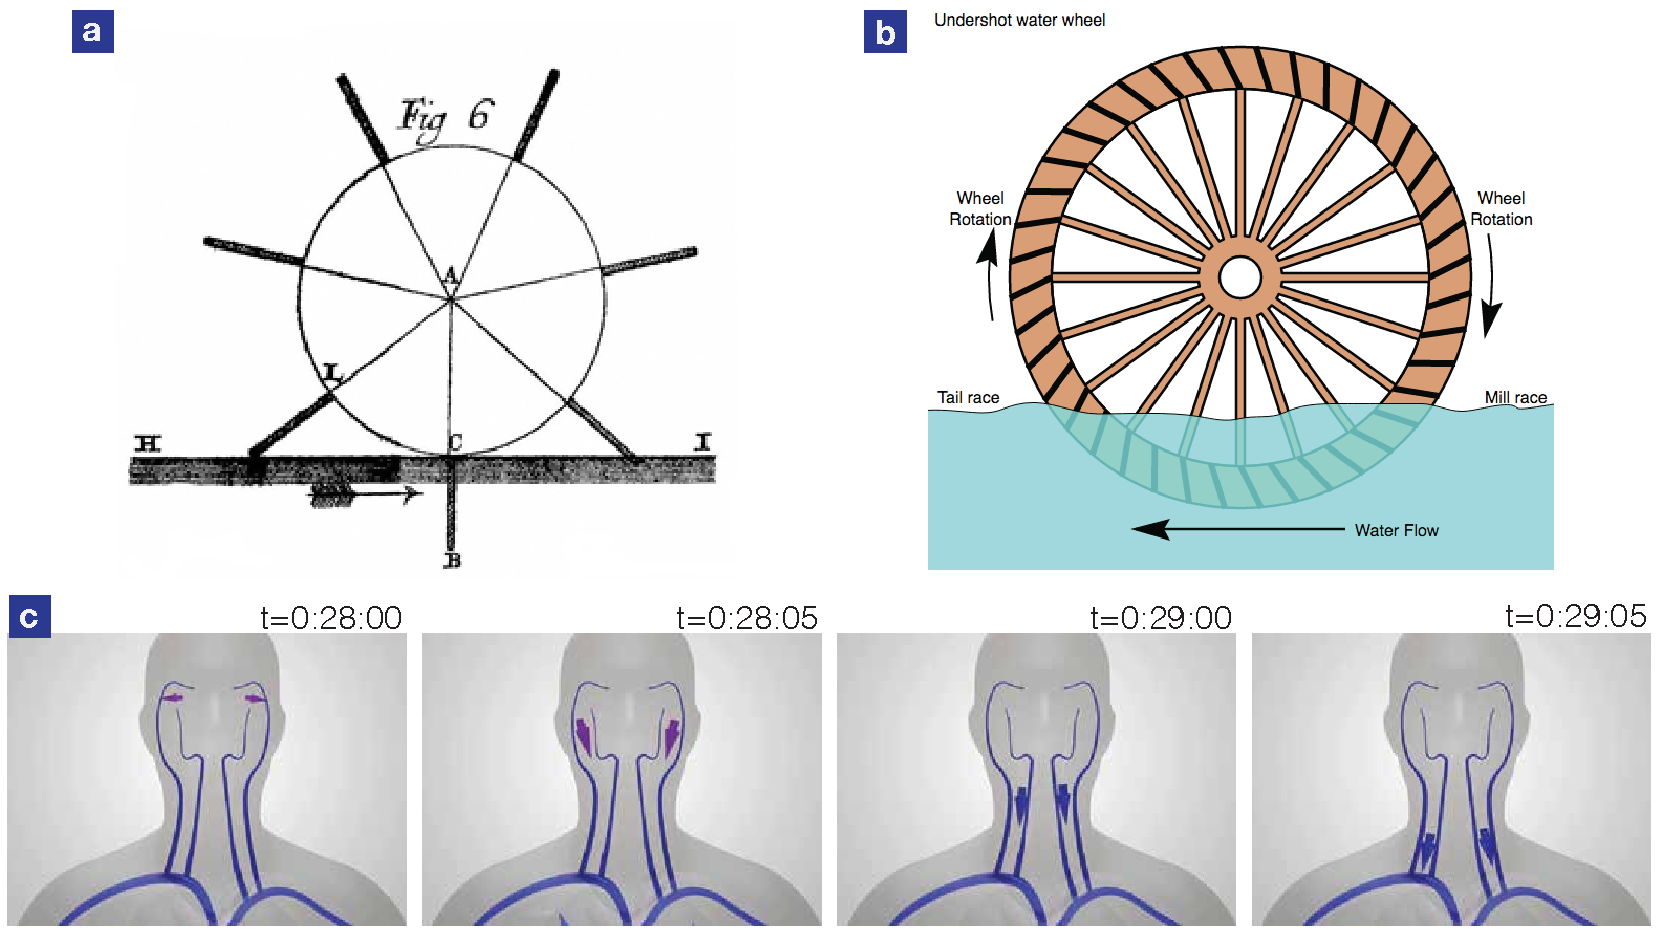
\includegraphics[width=0.6\textwidth]{\demowiz/fig/arrows/arrows}
  \caption{Three types of motion arrows in DemoWiz that guide presenters to the next event of different distances at a (A) far, (B) nearly the same, and (C) near location.}
  \label{fig:demowiz_arrows}
\end{figure*}

% --------------------------------------------------

\subsubsection{Sense of Timing}
DemoWiz provides a sense of timing for an upcoming action so that presenters can adjust their narration. First, DemoWizembeds \textit{a progress bar} in the motion arrow to show relative time (Figure~\ref{fig:demowiz_teaser}C). The green bar shows the proportional time that has been passed before reaching the next event (Figure~\ref{fig:demowiz_timing} top). When a motion arrow is filled up with green, it fades away and guides the presenter to the next action. We were concerned that people may associate the length of an arrow to the length of time. Therefore, we also incorporated a \textit{countdown} visualization where circles will fade out in the last three seconds before the next action starts (Figure~\ref{fig:demowiz_timing} bottom) to convey absolute timing.

\begin{figure*}[t]
  \centering
  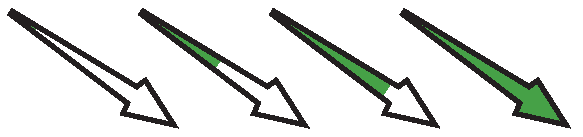
\includegraphics[width=0.6\textwidth]{\demowiz/fig/progressbar/progressbar}
  
\includegraphics[width=0.6\textwidth]{\demowiz/fig/countdown/countdown}
  \caption{A progress in time guides the presenter from the current event (left) gradually to the upcoming action (right) using relative timing with a progress bar (top) and absolute timing (bottom).}
  \label{fig:demowiz_timing}
\end{figure*}

% --------------------------------------------------

\subsubsection{Visualization Examples}
Figure~\ref{fig:demowiz_examples} presents examples of DemoWiz visualizations with four different systems. The glyphs effectively show the start and end points of mouse drags and the locations of mouse clicks. Motion arrows help direct the presenter's attention between events, such as start the end of the drag event to clicking a button (Figure~\ref{fig:demowiz_examples}A and B), clicking between several options (Figure~\ref{fig:demowiz_examples}C), or selecting a specific slide after scrolling down (Figure~\ref{fig:demowiz_examples}D).

\begin{figure*}[t]
  \centering
  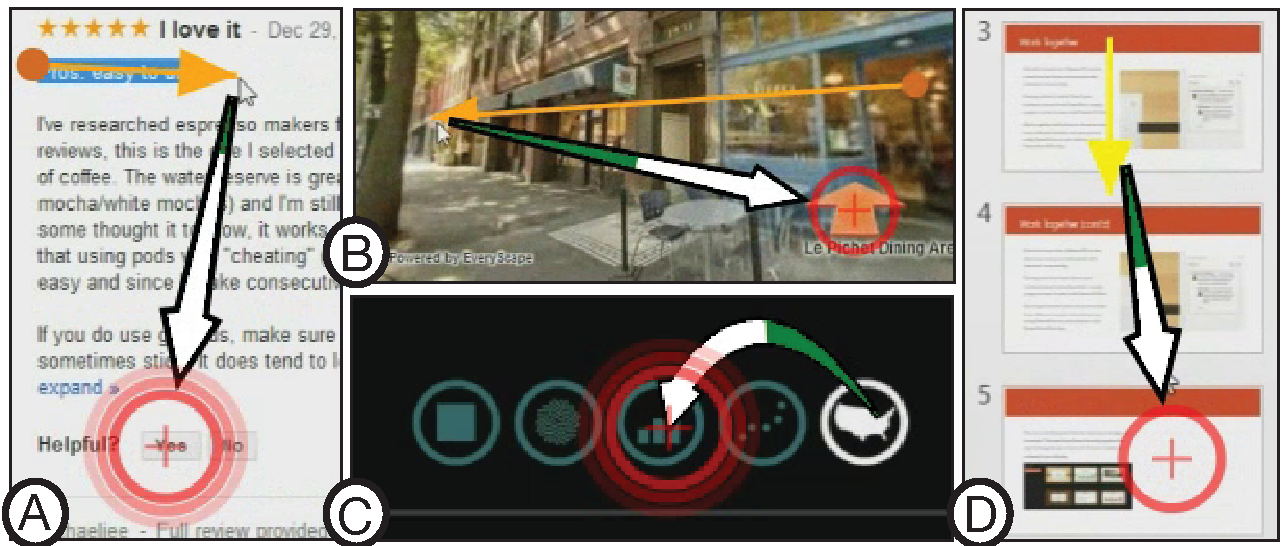
\includegraphics[width=0.7\textwidth]{\demowiz/fig/examples/examples}
  \caption{Examples of DemoWiz visualizations with four different systems and input event sequences.}
  \label{fig:demowiz_examples}
\end{figure*}

% ---------------------------------------------------------------

\subsection{Lightweight Editing During Rehearsal}
During rehearsal for their demonstration, presenters can modify the video timing and add reminder notes for their narration. DemoWiz shows the type and length of each event in a sequence in a timeline (Figure~\ref{fig:demowiz_teaser}A). Each segment is shown as a block whose width indicates its length in time. To simplify the timeline and avoid fine-grained adjustment,lengths of event blocks are rounded to the second. Presenters can modify the playback speed of a segment by dragging the boundaries of a segment on the timeline. For example, presenters can speed up to shorten long text inputs, and slowdown for fast mouse drag inputs that select multiple objects.

Sometimes a change in the playback speed may result in an awkward effect that is noticeable to the audience, especially when showing a UI transition. Therefore, DemoWiz supports two special time control markers to enable breaks in the narration. Presenters can add an adjustable \textit{pause} segment, at which the system will pause at the last frame of the previous segment for the specified length of time. If presenters prefer full control on pause length, a \textit{stop} marker ensures the video stays paused at the last frame of the previous segment and will not proceed until presenters manually resume the playback of the video.DemoWiz enables presenters to add a short text note (such as the reminder \iquote{Move and zoom...} in Figure~\ref{fig:demowiz_teaser}) so that they could remind themselves of upcoming actions at a higher level. The note can be positioned manually at any location on a video so that it does not block important video content, and will be shown for 3 seconds before the associated event.For every edit that is associated with time changes (including playback speed and pauses), DemoWiz computes and updates the total presentation time as well as updating the progress bar and countdown to provide accurate timing.

% ---------------------------------------------------------------

\subsection{Presenter View}
During presentation, DemoWiz shows two views in separate windows. Presenters can observe visualizations using the presenter view, while the audience will see the audience view with a full-screen video that has no enhanced information. DemoWiz synchronizes the videos in both views based on presenters' editing decisions to ensure the same playback speed and time. As with a conventional video player, presenters can control the video, to pause and play at any time. In addition, when a video is paused (or stopped), presenters can hover the mouse over the demo video in the presenter view to point out an important area, as many presenters currently do in a live demo. DemoWiz then simulates and synchronizes a mouse cursor in the audience view to help the audience follow the demonstration.

% ---------------------------------------------------------------

\subsection{Implementation Details}
During recording, DemoWiz captures the screen within a specified region and logs low-level system input data with\textit{timestamps} (with an accuracy of 0.1 seconds) from the operating system, including:

\begin{itemize}
  \item \textit{Mouse events} (mouse downs, mouse ups, and mouse wheel movements) and their \textit{positions} (in x-y coordinates relative to the screen-captured region).
  \item \textit{Key-press events} (keyboard input).
\end{itemize}

Once presenters finish their demonstrations, DemoWiz analyzes the low-level event stream and transforms it into high-level event metadata. For mouse events, we pair each mouse down and up into mouse \textit{clicks}, \textit{double-clicks}, or \textit{drags}. We group any consecutive mouse wheel events within a time threshold of 2 seconds to one \textit{scroll} event and any key-press events within the same threshold to one \textit{keystroke} event(e.g., combine keys d-o-w-n-t-o-w-n to ``downtown''). For each high-level event, we log the \textit{start} and \textit{end time} (timestamps of the first and the last low-level event).

Based on the start and end times of these high-level events, DemoWiz segments the screencast video recording into \textit{event segments}. Any gap between two consecutive input events is marked as an \textit{inactive segment}, which may include mouse hovering, UI transitions of the demo system, or static frames with no visual changes. DemoWiz adjusts the boundaries of these event segments to avoid any short visual effect that cannot be observed. DemoWiz examines segments in a linear order to ensure each segment lasts at least $t_{min}$ seconds long,which is set as one second based on our early testing. For an event segment $S_i$ of time ($t_{start}$, $t_{end}$) that $t_{end} - t_{start} < t_{min}$, DemoWiz expands 0.5 second forward and backward if $S_{i-1}$ and $S_{i+1}$ are inactive. If the adjusted $S_{i-1}'$ and $S_{i+1}'$ are shorter than $t_{min}$, DemoWiz merges it to the shorter neighbor segment. Currently, DemoWiz does not analyze these inactive segments, but techniques including computer vision and video analysis \cite{Banovic:2012kd,Chi:2012:MAG:2380116.2380130} can be applied for finer segmentation.

The capturing program is implemented in C\#. Two APIs were used: 1) the Windows Event Log API for mouse and keyboard hooks and 2) the Expression Encoder 4 API for screen recording running on Microsoft Windows 7. The recorded metadata(stored in a JSON object) and screencast video (in MP4) are read by the Presenter UI, which is implemented using standard Web technologies, including HTML5, CSS3, JavaScript, and jQuery. In particular, the visualization is rendered on the canvas element on top of the video object on the fly based on the video playback time. The audience view is generated by the main browser window of presenter view for video control.


%!TEX root = ../thesis.tex
\subsection{Implementation}
Kinectograph is implemented in C\# using the official Kinect API and the Arduino software. Our Tablet UI is implemented with the standard Web technologies, including HTML5, CSS3, JavaScript, and jQuery for recognizing touch gestures and communication.

% The tablet UI was built using HTML5/JavaScript. This communicated to t
% C\# program, Kinect API, Node.js server, HTML5/JavaScript web UI on iPad \pc{To write}


%!TEX root = ../thesis.tex
\section{Evaluation}
To evaluate the DemoWiz design, we conducted a controlled experiment in which participants recorded and edited a demo video, and gave a presentation with the edited video. Specifically, we wanted to see if presenters would evaluate their own performances higher with the support of our augmented visualizations and control of timing.

\subsection{User Study}

\subsubsection{Baseline Condition: DemoWiz without Visualization}
Since DemoWiz allows for rapid editing of the video, it would have been unfair to compare it with a conventional video player without supporting any editing during the rehearsal phase. We therefore modified our system to serve as the baseline condition, providing participants with the same lightweight editing of the video in each condition. However, during presentation, the baseline condition was similar to a conventional video player that shows only the video without event timeline and augmented visualizations. It also did not support the \textit{stop} markers and \textit{text notes}, i.e., participants could only adjust playback speed of each segment and add variable length \textit{pauses}. During presentation, participants only saw the video with a traditional timeline. They could, however, pause (or stop) and resume the video manually at any time during playback.

\subsubsection{Study Design}
We conducted the study as a within-subjects design in a usability room. After recording and editing a video using the same system, each presenter gave a presentation with both systems to an experimenter. To control the effect of order and learning, we prepared two tasks that included similar interaction flows and counterbalanced the order of the two systems—DemoWiz and Baseline—-but we fixed the order of tasks. Even though presenting to a single audience member in a usability room is not the same as using the system with a large conference audience, it is important to control the tasks and presentation as closely as possible to understand the relative benefits of the system in comparison with a baseline condition.

For each condition, we observed and coded the \textit{timing} of narration that matched the video content and noted the time in seconds when an event was described \textit{before}, \textit{at}, or \textit{after} the action happened in the demo video. We also marked obvious \textit{breaks} between narrations, \textit{errors} when the narration was not about the current or following events (e.g., discussing actions in a different order than they actually occurred), and \textit{misses} when an important action was not mentioned. To avoid unconscious bias that might influence the coding of the videos, we neutrally named the recordings and coded them all in a batch. We focused on objective timing measurements as much as possible, measuring deviation from specific video events and their corresponding narrations down to a second. Finally, we gathered qualitative feedback through satisfaction and preference questionnaires.

\subsubsection{Participants}
We recruited 12 participants (10 males and 2 females) from a software company. However, we excluded the data from two participants (1 male and 1 female); one was due to a software bug during one condition and another was because the participant requested to restart a presentation in one condition. The average age of the effective 10 participants was 37.3 ranging from 24 to 64 years of age. We recruited participants who had experience at showing a software demonstration to an audience such as giving a presentation at a conference. Four participants were native English speakers and the rest were fluent in English. The expertise of participants included audio processing, computer graphics, human-computer interactions, machine learning, networking, and software engineering. Each participant was compensated with lunch coupons worth \$20.

\subsubsection{Procedure and Tasks} Each session consisted of one training task and two experimental tasks. For the training task, to introduce the common features for recording and editing the video, we designed a simple workflow of five steps to demonstrate editing of a slide using PowerPoint. The experimenter briefly demonstrated an example and then introduced the recording program that captured the screen. Participants were then asked to practice and record using the recording program.

The two tasks consisted of a similar sequence and interactions: 1) searching with Bing Maps to show the 2D map view and the Bird's Eye view, looking for a restaurant, and navigating to the interior view of a specific restaurant; and 2) searching with Google Shopping to show the search results with the Grid view, filtering and voting for reviews, and navigating the 3D product view of an espresso machine. For each task, we provided a specific scenario along with a list of subtasks. The experimenter walked through this list with participants to ensure that they could easily find the features that needed to be demonstrated. Participants were then asked to practice (3-5 minutes), record (about 2 minutes), and rehearse and edit (5-10 minutes).

To help simulate a conference setting where participants would not be able to present immediately after having recorded a demonstration, we inserted an intentional 1-minute gap between rehearsal and presentation. During this gap before giving the presentation, we asked participants to watch a conference showcase video. Participants were then asked to stand up and gave a 2-3 minute presentation to the experimenter in a usability room.

After each task, participants filled out a questionnaire of 8-10 questions asking about their experience (8 for the Baseline condition, and 10 for the DemoWiz condition). At the end of the session, an online questionnaire was provided for them to present overall preferences and leave comments. Each session lasted about 1.5 hours.

\subsubsection{Experiment Setup}
Each participant used a desktop computer running Windows 7, Expression Encoder 4 for screen recording, and a web browser for the DemoWiz user interface. A regular mouse and keyboard were provided, along with two 27-inch displays, one for editing (during rehearsal) and showing the audience view (during presentation), and the other for the presenter view on a stand-up table. The resolution of both displays was 1920×1200 pixels. The average captured screen area was 1311×857 pixels. In the presenter view, the video resolution was within 1000×600 pixels; in the audience view, the screencast videos were resized to fill the entire display with at least 100-pixel wide border in black. During the study, the experimenter stayed in the room, providing instructions and sitting behind the participants during the recording and editing phases.

% ---------------------------------------------------------------

\subsection{Results}
Ten participants successfully recorded, rehearsed, and gave a demo with both systems.

\subsubsection{Subjective Preference}
Figure~\ref{fig:demowiz_likert} shows the average subject responses (on the 7-point Likert scale) from presenters for both systems. We analyzed these subjective responses using a Wilcoxon signed-rank test. We found significant differences in responses for ease of narration (DemoWiz µ = 6.2 over Baseline µ = 4.5, \textit{p} = .018) and ease of presentation (6.4 over 5.2, \textit{p} = .048). We also found marginally significant differences in participants' overall satisfaction with their presentations (5.5 over 4.7, \textit{p} = .062). Participants also tend to agree that DemoWiz helped them interpret timing (6.1 over 4.4, \textit{p} = .067).

In addition, 9 out of the 10 participants preferred DemoWiz to the system without visualization and would choose to present with DemoWiz if they were asked to give a public software demo; the remaining participant indicated no preference for both questions. The general feedback was also encouraging. For example, P1 commented \iquote{Awesome system. I'd use it today.} and P5 \iquote{felt more confident in being able to present what I wanted to.}

\begin{figure*}[t]
  \centering
  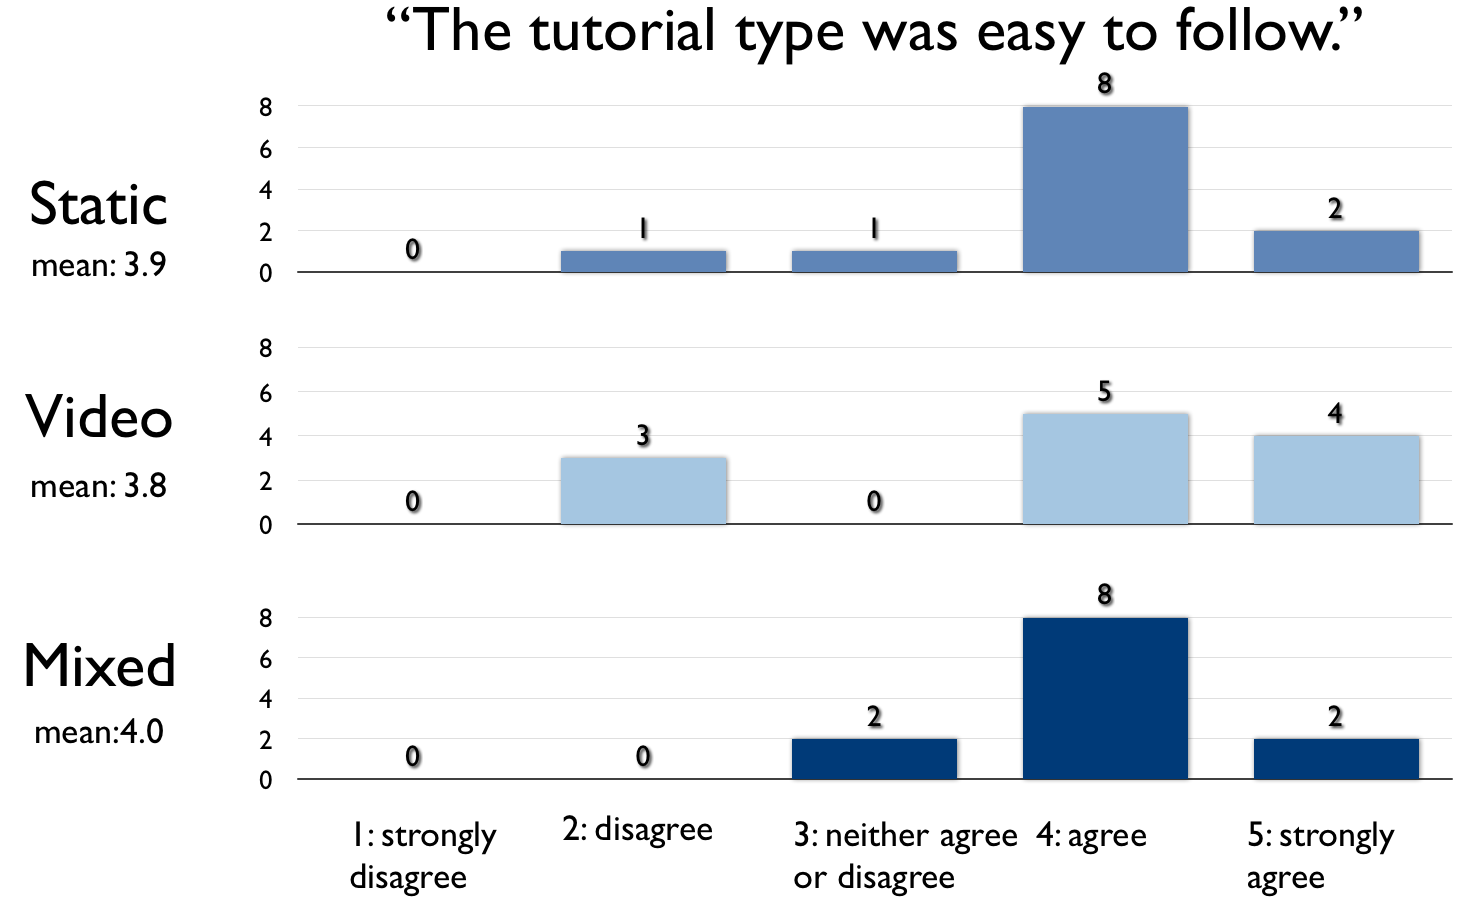
\includegraphics[width=\textwidth]{\demowiz/fig/results/likert}
  \caption{User feedback from questionnaire on the 7-point Likert scale.}
  \label{fig:demowiz_likert}
\end{figure*}

\subsubsection{Visualization as a Supportive Cue}
Participants answered that they were able to understand DemoWiz visualization of input events (µ = 6.0) and found it supportive for their presentations (µ = 6.3). They also commented that the DemoWiz visualization supported the presentation in various aspects: \iquote{the visualization reminds of the order of the content} (P1), \iquote{Really liked the ability to know what was coming up} (P2), \iquote{It provides better insight of the progress of the video} (P6), and \iquote{viz gave me an idea about timing or something I was going to forget to say} (P9).

\subsubsection{Narration Timing}
We coded the 20 recordings of participants' final presentations to observe the timing of narration of each action in correspondence with the video content (11 key events for both tasks). With DemoWiz, participants tended to \textit{anticipate} the upcoming events rather than talk afterwards, where the average timing was -0.1 seconds with DemoWiz (i.e., narrated the action before it happened) and 0.4 seconds with the Baseline condition (i.e., explained the action after it was shown). We found a significant difference in the number of times that events were anticipated by the narration, co-occurred, or occurred after the fact ($\chi $\textsuperscript{2}\textit{(2,220) = 8.6, p = .01}, see Figure~\ref{fig:demowiz_results_timing}).

In general, this supports our suspicion that DemoWiz would help in anticipating an event as opposed to talking about it after it occurred. More important though, was how often a narrator spoke about an event within several seconds of when the event actually occurred. By defining \textit{better} timing as when a presenter's explanation came within 2 seconds of a shown event (either prior, exact, or after), there was marginal significance by condition (\textit{p} = .089 with DemoWiz performing better). In addition, with the Baseline condition, the timing of narration was less consistent and off more, varying from 6 seconds early or 10 seconds late with a variance of 3.9 seconds, in comparison to the DemoWiz condition with at most 3 seconds early to 3 seconds late and a variance of 1.9 seconds.

Five participants had an obvious \textit{error} (forgot the next action or incorrectly narrated another action), had a long \textit{break} (waiting for more than 2 seconds until the action was made), or \textit{missed} an action (did not explain an important feature) when presenting with the Baseline condition. On the other hand, in the DemoWiz condition no errors were made, and there were only one long break and one miss from two different participants, respectively.

Participants' comments also support the fact that DemoWiz helped presenters anticipate the upcoming events. P7 explained, \iquote{(I) felt better able to time my speech to coincide with visual events, rather than trailing after them. Without the event visualizations, I felt like I was talking about what the audience had just seen, rather than having my words and visuals combine to a single message.}

\begin{figure*}[t]
  \centering
  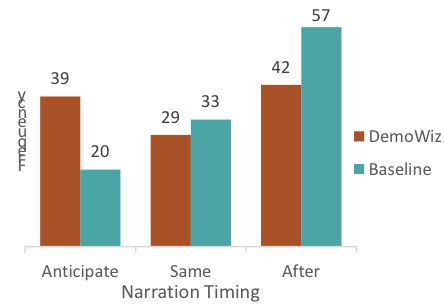
\includegraphics[width=\textwidth]{\demowiz/fig/results_timing}
  \caption{The number of times events were anticipated by the narration, co-occurred, or occurred after the fact.}
  \label{fig:demowiz_results_timing}
\end{figure*}

\subsubsection{Editing Experience}
We collected comments on the workflow. Participants found it easy to record (µ = 6.4) their demonstrations with DemoWiz. For editing features, they found it easy to edit in general (6.6), including controlling the playback speed (6.5) and adding pauses and stops (6.5), but it was less easy to add text notes (4.8); only two participants used this as reminders.

Although using different strategies, all of the participants adjusted the playback speed for matching their narration. Some sped up whenever possible and added stop markers for transitions; some slowed down the repetitive actions (such as drags) to demonstrate effects. P6 said, \iquote{I really liked being able to add ‘stop' events so I could \'fake\' my demo better.} DemoWiz made it easy for participants to separate the capturing and presentation preparation as P5 explained, \iquote{Overall, recording was very easy. In fact, as I got to the second task, I realized that I really don't need to think about the words as I record because later on I will be able to slow down and speed up time ...}

On average, the length of demo videos was 2'09\" before editing and 2'05\" after editing, and the presentation was 2'38\" long. Each participant spent 7.5 minutes on average to edit. For each demo of 44 segments on average, participants adjusted 3.15 segments for speedup and 4.25 segments for slowdown, and added 0.55 pause markers. In the DemoWiz condition, 1.2 stop markers and 0.2 text notes were added.


\section{Conclusion}
We presented Kinectograph, a new device that provides automatic and user-controlled camera orientation. We showed initial evidence of its effectiveness for self-recording demonstration tasks. We see applications of Kinectograph beyond the domain of instructional video and are investigating the opportunities of rich tracking information for video recording and editing in general.

%\section{Note on prior submission}
%This paper is based on a non-archival poster accepted for publication at CHI 2013. The prior version used a substantially different user interface and %backend. We also expanded the evaluation of our system in this submission.

% and whether the user's actions with the UI produced the expected result. we aimed to confirm that our features did work well and that the UI was easy enough to use to perform an assigned task.}

% Balancing columns in a ref list is a bit of a pain because you
% either use a hack like flushend or balance, or manually insert
% a column break.  http://www.tex.ac.uk/cgi-bin/texfaq2html?label=balance
% multicols doesn't work because we're already in two-column mode,
% and flushend isn't awesome, so I choose balance.  See this
% for more info: http://cs.brown.edu/system/software/latex/doc/balance.pdf
%
% Note that in a perfect world balance wants to be in the first
% column of the last page.
%
% If balance doesn't work for you, you can remove that and
% hard-code a column break into the bbl file right before you
% submit:
%
% http://stackoverflow.com/questions/2149854/how-to-manually-equalize-columns-
% in-an-ieee-paper-if-using-bibtex
%
% Or, just remove \balance and give up on balancing the last page.
%
